\scanpage{37}
\mspage{18}
\margin{Le passage de $u$ à $\tau(u)$ \unsure{s'effectue} par
\[
\begin{aligned}
\lambda&\longmapsto\varepsilon_0^{-1}(\tau_\infty(\lambda^{-1}))\\
(\lambda&\longmapsto\lambda\quad\text{si }\lambda=l_0^\gamma)\\
\eta&\longmapsto\tau_\infty(\eta)\\
\xi&\longmapsto\widetilde\sigma_\infty(\xi)=\sigma_\infty\tau_\infty(\xi)
\end{aligned}
\]}
\[
(63)\qquad\boxed{\boxed{\left\{\begin{aligned}
\beta'&=\alpha'\sigma_\infty(\lambda)\quad(=\alpha'l_1^\gamma\text{ si }\lambda=l_0^\gamma)\\
\text{avec}\qquad\alpha'&=\xi'\unsure{\rho|\rho^{-1}}(\xi')^{-1}\\
\beta'&=\eta\sigma_\infty(\eta)^{-1}
\end{aligned}\right.}}
\]
\margin{\uline{NB} L'\unsure{ens.} des relations stable par substitutions de la forme
\[
\begin{aligned}
\xi'&\longmapsto l_0^{\unsure{H|\mu}}\unsure{\xi|\xi\prime}\\
\eta&\longmapsto l_0^{\unsure{H|\mu}}\eta\\
\text{i.e.}\quad\alpha'&\longmapsto l_0^{\unsure{H|\mu}}\alpha'l_1^{-\unsure{H|\mu}}\\
\beta'&\longmapsto l_0^{\unsure{H|\mu}}\beta'l_1^{-\unsure{H|\mu}}
\end{aligned}
\]}
Ici, les quantités $\alpha',\beta',\xi'$ ont été introduites en termes des quantités primitives $\lambda,\eta,\xi$ $(\longmapsto\beta,\deleted{\unsure{\alpha}}\alpha,\widetilde\alpha)$, s'introduisant ds les formules (54) (et (57)), par le pur calcul \deleted{en} \inserted{dans} $\widehat\Pi_{0,3}$, comme donnant lieu aux formules les plus symétriques. Mais on peut les interpréter aussi de façon ``géométrique'', en posant (\deleted{\unsure{avant}} pour ce qui est de $\beta',\alpha',\widetilde\alpha'$)
\[
(64)\qquad\begin{aligned}
b_i^{\prime\omega}&=(b_i^\omega)^{-1}=b_i^{\omega'},\qquad
\unsure{(}\widetilde b_i^{\prime\omega}=(\widetilde b_i^\omega)^{-1},\qquad
\widetilde a_i^{\prime\omega}=(\widetilde a_i^\omega)^{-1}
\end{aligned}
\]
de sorte que les formules (57) deviennent
\[
(65)\qquad\left\{\begin{aligned}
u(b_i^{\prime\omega})&=\varphi_{\omega i}^\omega(\beta')b_i^{\prime\omega}\\
u(\widetilde b_i^{\prime\omega})&=\varphi_{\omega i}^\omega(\alpha')\widetilde b_i^{\prime\omega}\\
u(\widetilde a_i^{\prime\omega})&=\widetilde a_i^{\prime\omega}\psi_{\omega i}^\omega(\widetilde\alpha')
\end{aligned}\right.
\]
Enfin, la quantité $\xi'=\eta\xi$ est obtenue géométriquement, en introduisant les chemins
\diagram{\begin{tikzcd}[ampersand replacement=\&,column sep=large,row sep=large]
P^\omega\arrow[rr,"\widetilde d_i^{\prime\omega}"]\arrow[dr,"d_{\omega i}^\omega"']\&\&R_i^{\omega'}\\
\&Q_{\omega i}\arrow[ur,"c_{\omega i}^\omega"']\&
\end{tikzcd}}\quad(66)
\[
\widetilde d_i^{\prime\omega}=c_{\omega i}^\omega\cdot d_{\omega i}^\omega
\]
\figure{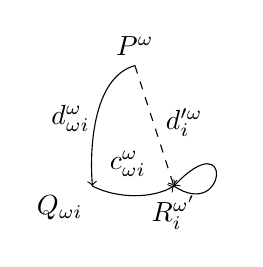
\begin{tikzpicture}[scale=.9]
\coordinate (P) at (.6,1.7);\coordinate (Q) at (0,0);\coordinate (R) at (1.15,0);
\draw[->] (P)..controls (.05,1.55) and (-.05,.65)..(Q);
\draw[dashed,->] (P)--(R);\draw[->] (Q)..controls (.35,-.18) and (.85,-.18)..(R);
\draw[->] (R)..controls (1.9,-.5) and (2,.9)..(R);
\node[above] at (P) {$P^\omega$};\node[below left] at (Q) {$Q_{\omega i}$};\node[below] at (R) {$R_i^{\omega'}$};
\node[left] at (.1,.95) {$d_{\omega i}^\omega$};\node[right] at (.9,.9) {$d_i^{\prime\omega}$};\node[above] at (.5,0) {$c_{\omega i}^\omega$};
\end{tikzpicture}}
par la formule
\margin{36}
